% !Mode:: "TeX:UTF-8:Hard"
\documentclass{beamer}
\usepackage[UTF8,indent]{ctexcap}
\usetheme{Madrid}%Madrid,JuanLesPins,Ilmenau
\usefonttheme[onlymath]{serif}

\newcommand\Emph{\textbf}

\AtBeginSection[]{
  \begin{frame}
  \vfill
  \centering
  \begin{beamercolorbox}[sep=8pt,center,shadow=true,rounded=true]{title}
    \usebeamerfont{title}\insertsectionhead\par%
  \end{beamercolorbox}
  \vfill
  \end{frame}
}

\AtBeginSubsection[]{
  \begin{frame}
  \vfill
  \centering
  \begin{beamercolorbox}[sep=8pt,center,shadow=true,rounded=true]{title}
    \usebeamerfont{title}\insertsubsectionhead\par%
  \end{beamercolorbox}
  \vfill
  \end{frame}
}

\AtBeginSubsubsection[]{
  \begin{frame}
  \vfill
  \centering
  \begin{beamercolorbox}[sep=8pt,center,shadow=true,rounded=true]{title}
    \usebeamerfont{title}\insertsubsubsectionhead\par%
  \end{beamercolorbox}
  \vfill
  \end{frame}
}


\title{面向节能的单/多列车优化决策问题}
%\author{三峡大学\and 艾鑫\\ 武汉大学\and 杨志巧\\ 湖南大学\and 李金武}

\author[艾鑫、杨志巧、李金武]{艾鑫 \inst{1} \and 杨志巧 \inst{2} \and 李金武 \inst{3}}
\institute[三大、武大、湖大]{\inst{1} 三峡大学\hspace{1em}理学院 \and %
                      \inst{2} 武汉大学\hspace{1em}数学与统计学院 \and %
                      \inst{3} 湖南大学\hspace{1em}机械与运载工程学院}

\date{\today}

\begin{document}
\maketitle

\section{问题回顾}
\subsection{第一问、单列车节能运行优化控制问题}
\begin{frame}{问题回顾}{问题一、单列车节能运行优化控制问题}
\begin{description}
  \item[第一小问] 请建立计算速度距离曲线的数学模型,计算寻找一条列车从$A_6$站出发到
达$A_7$站的最节能运行的速度距离曲线,其中两车站间的运行时间为110秒
  \item[第二小问] 请建立新的计算速度距离曲线的数学模型,计算寻找一条列车从$A_6$站出
发到达$A_8$站的最节能运行的速度距离曲线,其中要求列车在$A_7$车站停站45秒,$A_6$站和$A_8$站间
总运行时间规定为220秒(不包括停站时间)
\end{description}
\end{frame}

\subsection{第二问、多列车节能运行优化控制问题}
\begin{frame}{问题回顾}{第二问、多列车节能运行优化控制问题}
\begin{description}
  \item[第一小问] 当100列列车以间隔$H={h_1,\cdots,h_{99}}$从$A_1$站出发,\Emph{追踪运行},依次经
  过$A_2$,$A_3$,……到达$A_{14}$站,中间在各个车站停战最少$D_{\min}$秒,最多$D_{\max}$秒。间隔$H$各
  分量的变化范围是$H_{\min}$秒至$H_{\max}$秒。请建立优化模型并寻找使所有列车运行总能耗最低的间隔H。
  要求第一列列车发车时间和最后一列列车的发车时间之间间隔为$T_0=63900$秒,且从$A_1$站到$A_{14}$站的
  总运行时间不变,均为$2086$秒(包括停站时间)。假设所有列车处于同一供电区段。
\end{description}
\end{frame}

\begin{frame}{问题回顾}{第二问、多列车节能运行优化控制问题}
\begin{description}
  \item[第二小问] 接上问,如果高峰时间(早高峰$7200$秒至$12600$秒,晚高峰$43200$至$50400$秒)发车间隔
  不大于$2.5$分钟且不小于$2$分钟,其余时间发车间隔不小于$5$分钟,每天$240$列。请重新为它们制定运行图和相应
  的速度距离曲线。
\end{description}
\end{frame}

\subsection{第三问、列车延误后运行优化控制问题}
\begin{frame}{问题回顾}{第三问、列车延误后运行优化控制问题}
\begin{description}
  \item[第一小问] 接上问,若列车$i$在车站$A_j$延误$DT_j^i$(10秒)发车,请建立控制模型,找出在确保安全的前提下,首先使所有后
续列车尽快恢复正点运行,其次恢复期间耗能最少的列车运行曲线
  \item[第二小问] 假设$DT_j^i$为随机变量,普通延误($0<DT_j^i <10 \, \mathrm{s}$)概率为$20\%$,严重延误($DT_j^i >10 \, \mathrm{s}$)概率为$10\%$(超
过$120$秒,接近下一班,不考虑调整),无延误($DT_j^i= 0$)概率为$70\%$。若允许列车在各站到、发时间与原时
间相比提前不超过$10$秒,根据上述统计数据,如何对第二问的控制方案进行调整?
\end{description}
\end{frame}

\section{问题求解}
\subsection{第一问、单列车节能运行优化控制问题}
\subsubsection{模型建立}
\begin{frame}{目标函数的确定}
题设给出的目标是使得耗能最少,根据题设可知耗能主要是由于列车行驶需要牵引力,导致发电机就处于耗能状
态。查阅相关参考文献[2]可知在整个运行过程中所消耗的能量由牵引力来决定,如下所示:
\[E = \int_0^{{t_{\max }}} {F\left( t \right){v_t}dt} \]

注:${t_{\max }} = 110$ ,因为总的运行时间为110 秒。
\end{frame}

\begin{frame}{约束条件的确定}
约束条件一:由题目所给的数据中可以知道从 $A_6$站到 $A_7$站的总路程为1354m,因此整个过程中行走的总路程${L_{\max }} = 1354$ m,即:
\[\int_o^{{t_{\max }}} {{v_t}dt}  = {L_{\max }}\]
\\
约束条件二:列车起始时刻和到达 $A_7$站时刻的速度均为0且在运行的任何时刻速度都不能大于该时刻所处路段的最大速度$\overline {{v_t}} $ ,即:
\[\left\{ \begin{array}{l}
 {v_0} = {v_{{t_{\max }}}} = 0 \\
 {v_t} \le \overline {{v_t}}  \\
 \end{array} \right.\]
\\
约束条件三:由牛顿学第二定律可知,实际输出的牵引加速度乘以质量等于合外力,即:
\[m{a_t} = m\frac{{d{v_t}}}{{dt}} = F\left( t \right) - B\left( t \right) - W\left( t \right)\]
\end{frame}

\begin{frame}{第一问模型}
 综上所述,建立的单列车两个站点之间的最优化模型为:
\[\min {\kern 1pt} {\kern 1pt} {\kern 1pt} {\kern 1pt} {\kern 1pt} {\kern 1pt} {\kern 1pt} {\kern 1pt} {\kern 1pt} {\kern 1pt} E = \int_o^{{t_{\max }}} {F\left( t \right){v_t}dt} \]
\[s.t.\left\{ \begin{array}{l}
 \int_o^{{t_{\max }}} {{v_t}dt}  = {L_{\max }} \\
 \left\{ \begin{array}{l}
 {v_0} = {v_{{t_{\max }}}} = 0 \\
 {v_t} \le \overline {{v_t}}  \\
 \end{array} \right. \\
 m{a_t} = m\frac{{d{v_t}}}{{dt}} = F\left( t \right) - B\left( t \right) - W\left( t \right) \\
 F\left( t \right) = {k_t}{F_{\max }}\left( t \right) \\
 B\left( t \right) = {k_b}{B_{\max }}\left( t \right) \\
 W\left( t \right) = \left[ {{w_0}\left( t \right) + {w_1}\left( t \right)} \right] \times g \times {m \mathord{\left/
 {\vphantom {m {1000}}} \right.
 \kern-\nulldelimiterspace} {1000}} \\
 \end{array} \right.\]

\end{frame}

\subsubsection{求解算法}
\begin{frame}{换一个角度看问题}

\begin{itemize}
  \item<1-> 题目要求在给定的时间内,使消耗的能量最小
  \item<2-> 给定时间让能量最小$\Longrightarrow$ 比较困难
  \item<3-> 给定能量让时间最小$\Longrightarrow$ 容易求解
  \item<4-> 可以将第一个问题转化为第二个问题,首先构造一个能量比较小的初始解,然后不断的增加能量,直到时间
  满足要求
\end{itemize}
\end{frame}

\begin{frame}{为什么能够这么做?}
    \begin{columns}[c]
        \column{8cm}
            \begin{itemize}
              \item 将此问题推广为一个多目标规划问题
                \begin{itemize}
                  \item 目标一:$\min \quad t$
                  \item 目标二:$\min \quad E$
                \end{itemize}
              \item 运行方案$(t,E) \Longrightarrow  P(t,E)$
              \item 多目标规划:Pareto front $C$(非劣解集)
            \end{itemize}
        \column{5cm}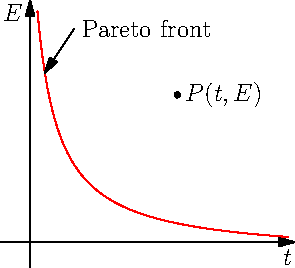
\includegraphics[width=4.5cm]{fig/fig1/fig1.pdf}
    \end{columns}
\end{frame}

\begin{frame}{为什么能够这么做?}
    \begin{columns}[c]
        \column{8cm}
            \begin{itemize}
              \item 原问题:给定时间$t_n$,求$E_{\min}$ $\Longrightarrow$ 求$t = t_n$与$C$的交点对应的运行方案
              \item 如果我们能够给出能量较小的初始解$(t_1,E_1)$,然后逐步添加能量,直到$t = t_n$,即求得原问题的运行方案
            \end{itemize}
        \column{5cm}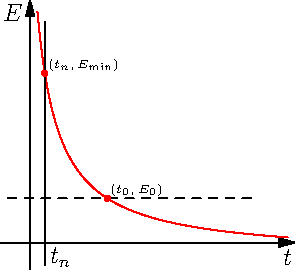
\includegraphics[width=4.5cm]{fig/fig2/fig2.pdf}
    \end{columns}
\end{frame}

\begin{frame}{为什么能够这么做?}
    \begin{columns}[c]
        \column{8cm}
            \begin{itemize}
              \item 原问题:给定时间$t_n$,求$E_{\min}$ $\Longrightarrow$ 求$t = t_n$与$C$的交点
              \item 如果我们能够给出能量较小的初始解$(t_1,E_1)$,然后逐步添加能量,直到$t = t_n$
            \end{itemize}
        \column{5cm}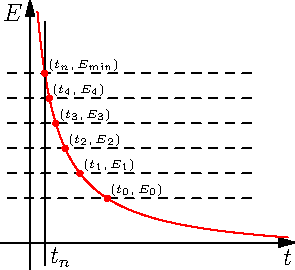
\includegraphics[width=4.5cm]{fig/fig3/fig3.pdf}
    \end{columns}
\end{frame}

\begin{frame}{考虑一个理想的情况}
\begin{columns}[c]
    \column{5cm}
        下面考虑一个理想的情况,即假设:
        \begin{itemize}
          \item 速度限制$v_{\max}$为常数
          \item 阻力$r$也为常数
        \end{itemize}
    \column{6cm}
    \begin{block}{优化模型}
        \begin{equation*}
          \min \quad E = \int_0^{t_{\max}} k_t(t) v(t) F(t) dt
        \end{equation*}
        \begin{equation*}
          s.t. \left\{
          \begin{array}{l}
            m \frac{dv(t)}{dt} = k_t F - k_b B - r \\
            L = \int_0^{t_{\max}} v(t) dt \\
            v(0) = v_0, \quad v(t_{\max}) = v_T \\
            k_t \in [0, 1], k_b \in [0,1], v \leq v_{\max}
          \end{array}
          \right.
        \end{equation*}
    \end{block}
\end{columns}
\end{frame}

\begin{frame}{Pontryagin最大值原理}
\begin{columns}[c]
    \column{6.5cm}
        根据Pontryagin最大值原理,前述优化模型可以转化为最大化下面的哈密顿函数:
        \begin{equation*}
          H = \frac{p_1}{v} \times (k_t F - k_b B - r) + p_2 v - k_t v F
        \end{equation*}
        其中$p_1$应该满足下面的微分方程:
        \begin{equation*}
          \frac{dp_1}{ds} = - \frac{\partial H}{\partial v}
        \end{equation*}
    \column{5.5cm}
    \begin{block}{求解结果}
    \begin{equation*}
      \left\{
        \begin{array}{l}
        k_t = 1, k_b = 0, \, (p_1>v^2) \\
        k_t \in [0,1], k_b = 0, \, (p_1 = v^2) \\
        k_t = 0, k_b \in [0,1], \, (p_1 = 0) \\
        k_t = 0, k_b = 0, \, (0 < p_1 < v^2) \\
        k_t = 0, k_b = 1, \, (p_1 < 0).
        \end{array}
      \right.
    \end{equation*}
    \end{block}
\end{columns}
\end{frame}

\begin{frame}{Pontryagin最大值原理}
\begin{columns}[c]
\column{5cm}
求解结果与四个阶段相对应:
\begin{description}
  \item[最大加速] $k_t = 1, k_b = 0$
  \item[巡航] $k_t \in [0,1], k_b = 0$
  \item[巡航] $k_t = 0, k_b \in [0,1]$
  \item[惰行] $k_t = 0, k_b = 0$
  \item[最大制动] $k_t = 0, k_b = 1$
\end{description}

\column{7cm} 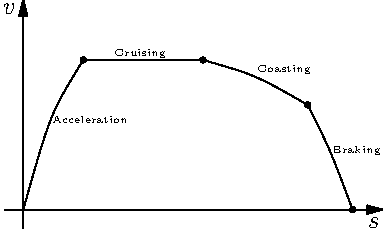
\includegraphics[width=7cm]{fig/fig4/fig4.pdf}
\end{columns}
\end{frame}

\begin{frame}{Pontryagin最大值原理}
\begin{columns}[c]
\column{8cm}

\begin{block}{最大值原理结论}
对于理想情况,所有“能量最小”和“时间最短”问题的最优解都是由:最大牵引、巡航、惰行和最大制动组成。
\end{block}

\column{4.2cm} 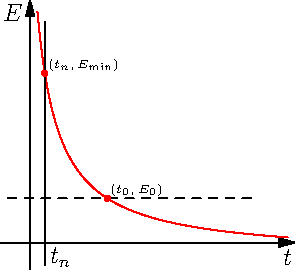
\includegraphics[width=4cm]{fig/fig2/fig2.pdf}
\end{columns}
\end{frame}

\begin{frame}{回到实际情况}
%\begin{columns}[c]
%\column{6cm}
\begin{itemize}
  \item 实际情况下,不同路段的速度限制是不一样的
  \item 实际路况(坡度、曲率)是随着路段变化的
  \item 基本阻力与速度相关
\end{itemize}
%\column{6cm}
\begin{center}
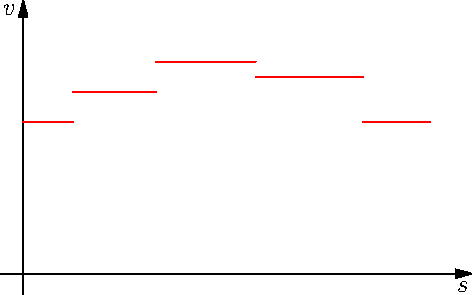
\includegraphics[width=7cm]{fig/fig5/fig5.pdf}
\end{center}
%\end{columns}
\end{frame}

\begin{frame}{求解初始解}
\begin{block}{初始解求法}
首先将列车最大加速到速度为$50 \mathrm{km/h}$,然后使列车惰行,在要到达终点时按最大制动进行制动。
\end{block}
\begin{itemize}
  \item 加速到$50 \mathrm{km/h}$是因为一般速度限制都大于等于$50 \mathrm{km/h}$
  \item 实际过程中发现,部分路段阻力过大,因此在惰行的时候要设置一个加速度下限
  \item 具体的制动点是通过检测是否遇到制动曲线来确定的
\end{itemize}
\end{frame}

\begin{frame}{制动点的确定}
\begin{block}{什么是制动曲线?}
制动曲线是在某一点,以该点的目标速度按照最大制动逆推出来的速度-路程曲线。在列车行驶过程中,一旦列车的
速度-路程曲线遇到制动曲线就要立刻进行最大制动。
\end{block}

\begin{center}
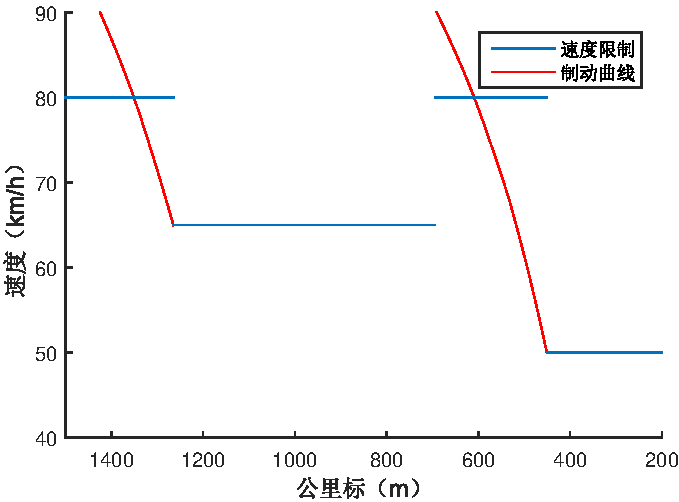
\includegraphics[width=6.5cm]{fig/fig6/fig6.pdf}
\end{center}
\end{frame}

\begin{frame}{一个实际的初始解}
\begin{center}
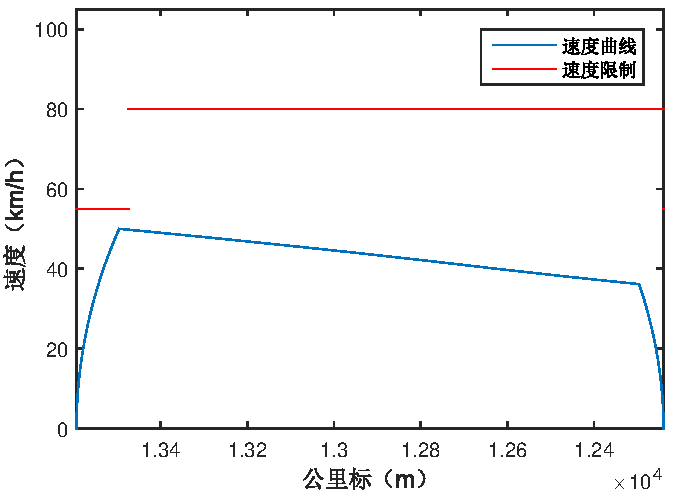
\includegraphics[width=8cm]{fig/fig7/fig7.pdf}
\end{center}
\end{frame}

\begin{frame}{初始解的逐步修正}
得到初始解后,以速度限制对路程进行分区,使得在每个分区内的速度限制都是一样的。

\begin{center}
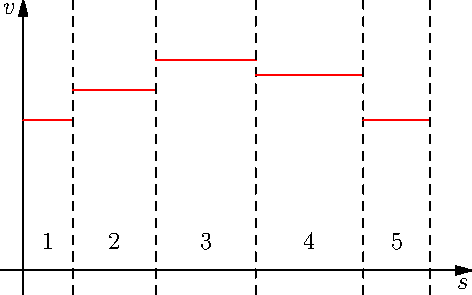
\includegraphics[width=8cm]{fig/fig8/fig8.pdf}
\end{center}
\end{frame}

\begin{frame}{初始解的逐步修正}
一般得到的初始解的时间是大于所规定的运行时间,所以需要多分配一小份能量$\Delta E$,对初始解进行逐步
修正,直到达到目标运行时间为止。

\begin{block}{能量分配准则}
设总路程按照速度限制分成了$N$个子区间,逐次将分配的能量$\Delta E$分配到各个子区间。对于分配能量的区间
按照已分配到的总能量,按照:最大加速、巡航、惰行、最大制动的策略计算运行方案。因此可以得到每一个区间
的节省时间$\Delta t_i$,将能量$\Delta E$分配给节省时间最多的区间。
\end{block}
\end{frame}

\begin{frame}{多站点情况}
\begin{itemize}
  \item 对于多站点情况,可以看做是两站点情况的一个特例
  \item 对于初始解,可以先生成相邻两个站点之间的初始解,拼接起来形成多站点情况的初始解
  \item 在相邻两个站点之间任然按照速度限制划分子区间,将所有子区间都当做多站点情况的子区间。逐步优化初始解
  过程与之前一样
\end{itemize}
\end{frame}

\begin{frame}{第一问速度路程曲线}{第一小问}
\begin{center}
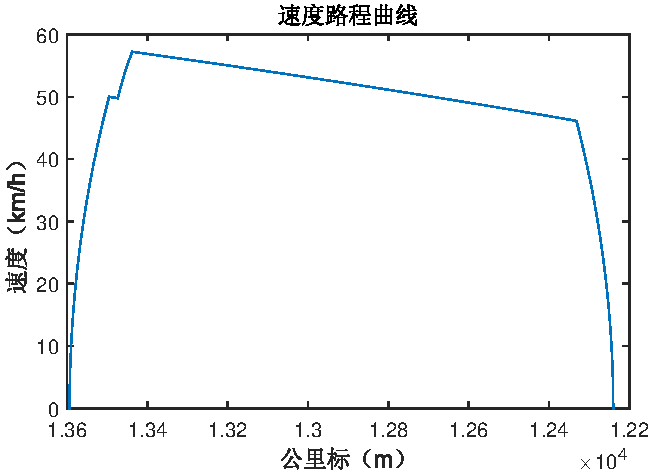
\includegraphics[width=9cm]{fig/fig9/fig9.pdf}
\end{center}
\end{frame}

\begin{frame}{第一问速度路程曲线}{第二小问}
\begin{center}
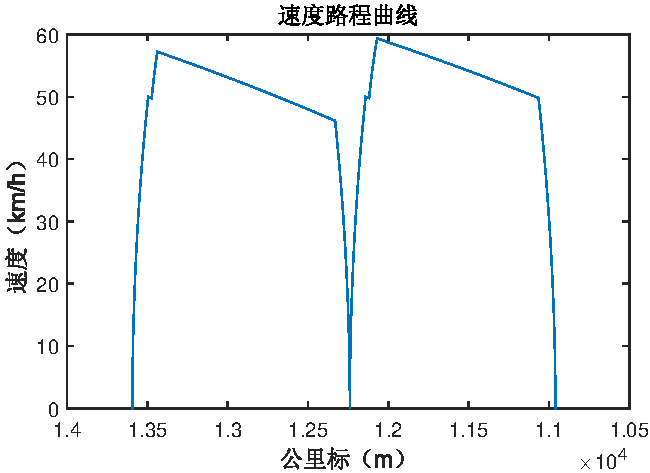
\includegraphics[width=9cm]{fig/fig10/fig10.pdf}
\end{center}
\end{frame}


\subsection{第二问、多列车节能运行优化控制问题}

\begin{frame}{问题回顾}{第二问、多列车节能运行优化控制问题}
\begin{description}
  \item[第一小问] 当100列列车以间隔$H={h_1,\cdots,h_{99}}$从$A_1$站出发,\Emph{追踪运行},依次经
  过$A_2$,$A_3$,……到达$A_{14}$站,中间在各个车站停战最少$D_{\min}$秒,最多$D_{\max}$秒。间隔$H$各
  分量的变化范围是$H_{\min}$秒至$H_{\max}$秒。请建立优化模型并寻找使所有列车运行总能耗最低的间隔H。
  要求第一列列车发车时间和最后一列列车的发车时间之间间隔为$T_0=63900$秒,且从$A_1$站到$A_{14}$站的
  总运行时间不变,均为$2086$秒(包括停站时间)。假设所有列车处于同一供电区段。
\end{description}
\end{frame}

\begin{frame}{问题分析}
\begin{itemize}
  \item<1-> 第二问考虑的是一个多列车节能优化运行问题
  \item<2-> 对于多个列车,如果一起考虑必然非常复杂。题目中提到一个词:“追踪运行”。因此我们让每个列车的
  行驶方案一致,不同的仅仅只是各列车的发车间隔和停留间隔
  \item<3-> 事实上,同时考虑发车间隔和站点停留间隔,这个问题也很复杂,因此令每个列车的停留时间相同,只
  考虑发车间隔的优化。
  \item<4-> 本文需要考虑再生能量的利用问题,所以发车间隔的优化的目的就是尽可能的利用再生能量
  \item<5-> 于是本问题分解为两个问题
    \begin{itemize}
        \item<6-> 单个列车的优化问题,使单个列车消耗的能量尽可能的少
        \item<7-> 各列车的发车间隔优化问题,使利用的再生能量尽可能的多
    \end{itemize}
\end{itemize}

\end{frame}

\begin{frame}{单个列车的优化问题}
单个列车的优化问题在第一问中已经解决了,利用第一问的算法,求出的从站点$A_1$到$A_{14}$的速度路程曲线为:

\begin{center}
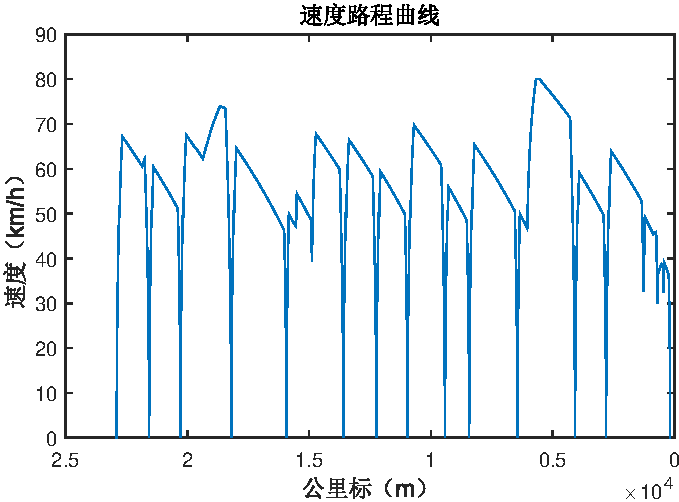
\includegraphics[width=8.3cm]{fig/fig11/fig11.pdf}
\end{center}
\end{frame}

\begin{frame}{再生能量的利用}

\begin{block}{再生能量}
列车在制动时会产生能量$E_{reg}$,如果有其余车辆处于加速状态,其可以利用能量$E_{reg}$。产生的再生能量为:
$$E_{reg} = (E_{mech} - E_f) \cdot 95 \%$$
其中$E_{mech}$为机械能的变化量,$E_f$为克服基本阻力和附加阻力做的功。
\end{block}

再生能量的利用按照下面的公式计算:
$$E_{used} = E_{reg} \cdot \frac{t_{overlap}}{t_{brake}}$$

\end{frame}

\begin{frame}{再生能量利用示意图}
\begin{center}
图:再生能量利用示意图
\end{center}

\end{frame}

\begin{frame}{发车间隔的优化}

\begin{description}
    \item[目标函数] 由于单个列车消耗的能量已经确定,并且各列车的形式方案一致,故各列车消耗的能量为
    一个定值。因此我们的目标就是让利用的再生能量最大
    \item[优化方法] 每两个列车之间有一个发车间隔,所有总共有99个自变量,并且目标函数的计算过程比较
    复杂,无法使用传统的优化算法求解。在此我们采用遗传算法进行求解
\end{description}

\end{frame}

\begin{frame}{第二问第一小问结果}
\begin{center}
图:第二问第一小问结果
\end{center}
\end{frame}

\begin{frame}{结果的一点解释}

为什么发车间隔都差不多?原因是:
\begin{itemize}
    \item 题目要求第一列列车发车时间和最后一列列车的发车时间之间间隔为63900秒
    \item 平均下来发车间隔为645秒左右
    \item 发车间隔的最大值限制为11分钟,即660秒
    \item 因此没有多大的调整空间
\end{itemize}

\end{frame}

\begin{frame}{问题回顾}{第二问、多列车节能运行优化控制问题}
\begin{description}
  \item[第二小问] 接上问,如果高峰时间(早高峰$7200$秒至$12600$秒,晚高峰$43200$至$50400$秒)发车间隔
  不大于$2.5$分钟且不小于$2$分钟,其余时间发车间隔不小于$5$分钟,每天$240$列。请重新为它们制定运行图和相应
  的速度距离曲线。
\end{description}
\end{frame}

\begin{frame}{第二问第二小问分析}
第二小问与第一小问的差别是
\begin{itemize}
    \item 在早高峰和晚高峰增加了特殊的发车间隔限制
    \item 发车量变为240列
\end{itemize}
面临的困难:
\begin{itemize}
    \item 高峰时期的限制不好添加。哪些列车处于高峰期,取决于前面列车的发车间隔。无法明确指定对某一变量的
    限制
    \item 自变量的数目变得更多,目标函数的计算量更大
\end{itemize}
\end{frame}

\begin{frame}{第二小问算法}{蒙特卡洛法}
【第二小问思路介绍】
\end{frame}

\begin{frame}{第二小问结果}
【第二小问结果】
\end{frame}

\subsection{第三问、列车延误后运行优化控制问题}
\begin{frame}{问题回顾}{第三问、列车延误后运行优化控制问题}
\begin{description}
  \item[第一小问] 接上问,若列车$i$在车站$A_j$延误$DT_j^i$(10秒)发车,请建立控制模型,找出在确保安全的前提下,首先使所有后
续列车尽快恢复正点运行,其次恢复期间耗能最少的列车运行曲线
  \item[第二小问] 假设$DT_j^i$为随机变量,普通延误($0<DT_j^i <10 \, \mathrm{s}$)概率为$20\%$,严重延误($DT_j^i >10 \, \mathrm{s}$)概率为$10\%$(超
过$120$秒,接近下一班,不考虑调整),无延误($DT_j^i= 0$)概率为$70\%$。若允许列车在各站到、发时间与原时
间相比提前不超过$10$秒,根据上述统计数据,如何对第二问的控制方案进行调整?
\end{description}
\end{frame}

\begin{frame}{问题分析}
\begin{itemize}
  \item 首先要保证列车的安全,后车的速度不能超过限制速度$V_{limit} = min(V_{line}, \sqrt{2LB_e})$
  \begin{itemize}
    \item $V_{line}$是列车当前位置的速度限速($ \rm km/h$)
    \item $L$是当前时刻前后车之间的距离($\rm m$)
    \item $B_e$是列车制动的最大减速度($\rm m/s^2$)
  \end{itemize}
  \item 然后要尽快恢复正点运行,最后才考虑能耗最少
  \item 下面我们分两种情况考虑这个问题
\end{itemize}
\end{frame}

\begin{frame}{小延误情况}
\begin{block}{小延误情况}
小延误是指当前延误列车并不影响后续列车的情况。判断条件是当前延误列车与下一列列车的发车间隔大于最小
发车间隔。
\end{block}
\begin{itemize}
  \item<1-> 这种情况下,我们仅考虑延误的这一辆列车,让其尽可能的准时到达下一个站点
  \item<2-> 若无法准时到达下个站点,则让其尽可能准时的到达下下个站点,以此类推
  \item<3-> 为使能量消耗最小其中依然采用第一问的运行控制模型
\end{itemize}
\end{frame}

\begin{frame}{大延误情况}
\begin{itemize}
  \item<1-> 当延误时间过长的时候,可能会影响到后续列车的运行
  \item<2-> 对于这种情况,我们让延误的列车首先按照小延误的情况,尽可能快的恢复正点运行
  \item<3-> 若后续列车在预定的发车时间与前车发车的时间间隔小于最小发车
  间隔,则让其顺延,直到与前车的发车间隔大于最小发车间隔为止
  \item<4-> 在后续的运行过程中按照新的速度限制$V_{limit} = min(V_{line}, \sqrt{2LB_e})$运行
\end{itemize}
\end{frame}

\begin{frame}{第一小问结果}
对于第一小问,都是属于小延误情况,所以仅需考虑单个列车的延误。求解的结果如下:
\begin{center}
图:第三问第一小问结果
\end{center}
\end{frame}

\begin{frame}{第二小问结果}
第二小问考虑延误时间为随机变量,故采用计算机模拟的方法,按照题目的要求生成延误时间的随机数。
模拟的部分结果如下:
\end{frame}

\section{总结与展望}
\begin{frame}{总结}
\begin{description}
  \item[第一问]<1-> 将行程按照速度限制划分区间。构造能量较小的初始解,然后逐步添加能量对初始解进行修正,
  直到耗时达到给定时间
  \item[第二问]<2-> 先建立单个列车的最优行车方案,然后采用遗传算法对发车间隔进行优化。对于第二小问,用
  蒙特卡洛法进行求解
  \item[第三问]<3-> 分小延误和大延误两种情况,对于小延误仅考虑延误的单个列车,让其尽快的正点运行。对于大
延误,后续列车与延误列车的发车间隔必须大于最小发车间隔,并采用新的速度限制公式
\end{description}

\end{frame}

\begin{frame}{有待改进的地反}
\begin{itemize}
  \item<1-> 在第一问的算法中,可以考虑一次对两个区间进行修正
  \item<2-> 在第二问中可以考虑对停车间隔的优化
  \item<3-> 改进第二问第二小问的算法
  \item<4-> 考虑多个列车同时延误的情况
\end{itemize}

\end{frame}

\begin{frame}[c]
\begin{center}
\Huge 谢谢!
\end{center}
\end{frame}

\end{document}
